%%%%%%%%%%%%%%%%%%%%%%%%%%%%%%%%%%%%%%%%%
% Journal Article
% LaTeX Template
% Version 1.3 (9/9/13)
%
% This template has been downloaded from:
% http://www.LaTeXTemplates.com
%
% Original author:
% Frits Wenneker (http://www.howtotex.com)
%
% License:
% CC BY-NC-SA 3.0 (http://creativecommons.org/licenses/by-nc-sa/3.0/)
%
%%%%%%%%%%%%%%%%%%%%%%%%%%%%%%%%%%%%%%%%%

%----------------------------------------------------------------------------------------
%	PACKAGES AND OTHER DOCUMENT CONFIGURATIONS
%----------------------------------------------------------------------------------------

\documentclass[twoside]{article}
\usepackage{lipsum} % Package to generate dummy text throughout this template
\usepackage[superscript]{cite}
\usepackage[sc]{mathpazo} % Use the Palatino font
\usepackage[T1]{fontenc} % Use 8-bit encoding that has 256 glyphs
\linespread{1.05} % Line spacing - Palatino needs more space between lines
\usepackage{microtype} % Slightly tweak font spacing for aesthetics
\usepackage{amsthm}
\usepackage[margin=0.5in, top=30mm,columnsep=50pt]{geometry} % Document margins
\usepackage{multicol} % Used for the two-column layout of the document
\usepackage[hang, small,labelfont=bf,up,textfont=it,up]{caption} % Custom captions under/above floats in tables or figures
\usepackage{booktabs} % Horizontal rules in tables
\usepackage{float} % Required for tables and figures in the multi-column environment - they need to be placed in specific locations with the [H] (e.g. \begin{table}[H])
\usepackage{hyperref} % For hyperlinks in the PDF
\usepackage{graphicx}
\usepackage{lettrine} % The lettrine is the first enlarged letter at the beginning of the text
\usepackage{paralist} % Used for the compactitem environment which makes bullet points with less space between them
\usepackage{ulem}
\usepackage{empheq}
\newcommand*\widefbox[1]{\fbox{\hspace{2em}#1\hspace{2em}}}
\usepackage{amsmath}

\newtheorem*{hyp*}{Hypothesis}

\usepackage{abstract} % Allows abstract customization
\renewcommand{\abstractnamefont}{\normalfont\bfseries} % Set the "Abstract" text to bold
\renewcommand{\abstracttextfont}{\normalfont\small\itshape} % Set the abstract itself to small italic text

\usepackage{titlesec} % Allows customization of titles
\renewcommand\thesection{\Roman{section}} % Roman numerals for the sections
\renewcommand\thesubsection{\Roman{subsection}} % Roman numerals for subsections
\titleformat{\section}[block]{\large\scshape\centering}{\thesection.}{1em}{} % Change the look of the section titles
\titleformat{\subsection}[block]{\large}{\thesubsection.}{1em}{} % Change the look of the section titles

\usepackage{fancyhdr} % Headers and footers
\pagestyle{fancy} % All pages have headers and footers
\fancyhead{} % Blank out the default header
\fancyfoot{} % Blank out the default footer
\fancyhead[C]{Imperial College London$\bullet$ March 2014 $\bullet$ Henry O'Hagan } % Custom header text
\fancyfoot[RO,LE]{\thepage} % Custom footer text
\usepackage{perpage} %the perpage package
\MakePerPage{footnote} %the perpage package command



\usepackage{mathtools}
\DeclarePairedDelimiter\ceil{\lceil}{\rceil}
\DeclarePairedDelimiter\floor{\lfloor}{\rfloor}

%----------------------------------------------------------------------------------------
%	TITLE SECTION
%----------------------------------------------------------------------------------------

\title{\vspace{-15mm}\fontsize{18pt}{10pt}\selectfont\textbf{Self-Organised Criticality in the Oslo Model}\vspace{-15mm}} % Article title

\date{}

%----------------------------------------------------------------------------------------

\begin{document}
\normalem
\maketitle % Insert title

\thispagestyle{fancy} % All pages have headers and footers

%----------------------------------------------------------------------------------------
%	ABSTRACT
%----------------------------------------------------------------------------------------

\begin{abstract}

\noindent 
% results
This report will look into a system which display self-organised criticality, namely the Oslo model. Self organised criticality typically occurs in systems that are non-linear, and therefore sensitive to feedback from the system.After evolving through a transient period a self-organised critical system tends towards a steady state. These steady states are attractors of the dynamics, they are critical points where the system exhibits scale-free behaviour. Rice piles, which are slowly driven (i.e. only one grain is added until the pile settles) are systems which display self-organised criticality. If the system starts at an empty state it will self organise such that the number of grains added on average is equal to the number of grains leaving the system on average. As grains are added they tend towards an attractor where the avalanche sizes occur over all scales, limited only by the system size.
\end{abstract}

%----------------------------------------------------------------------------------------
%	ARTICLE CONTENTS
%----------------------------------------------------------------------------------------

{\let\thefootnote\relax\footnote{Word Count:2000}}

\vspace{-5mm}
\section{Aims \& Introduction}

\lettrine[nindent=0em,lines=2]{T}he Oslo model is a model of a rice pile which is defined by an algorithm which operates on a lattice. Each lattice site has a local slope associated with it. If the algorithm causes the slope to increase past a certain point it adjusts the slopes to become stable again. The algorithm first cycles through a set of transient configurations that is only visited once, and after some cross-over time the system will reach a steady state, at this point the system is cycling through the set of recurrent configurations. The aims are to investigate the height, cross-over times, the height during the steady states, the avalanche sizes during the steady states, and the number of grains leaving the system and how they scale with the system size.

%------------------------------------------------METHOD

\section{Methods}
\subsection{Oslo Model Algorithm\cite{cc}}
The algorithm is defined on a 1 dimensional lattice composed of $L$ sites, for site $i=1,2,\ldots,L$. The number of grains on site $i$ is given by the height at site $i$, $h_i \in \mathbb{Z}^+ \cup \{ 0 \}$. The local slope is defined by $z_i=h_i - h_{i+1}$, where $h_{L+1} = 0$. Each site is assigned a threshold slope $z_i^{th} \in \{ 1, 2 \}$ with a probabilities $P(z_i^{th} = 1) = p$, and $P(z_i^{th} =2) = 1-p$ . The system is driven by adding grains at site $i=1$, allowing it to completely relax into a new configuration before adding another. Site $i$ relaxes if $z_i^{th}<z_i$, then one grain topples from site $i$ to site $i+1$. i.e. $h_i \to h_i -1$, $h_{i+1} \to h_{i+1} +1$. In terms of local slopes, the algorithm used is as follows:
\begin{enumerate}
\item Prepare the system such that $z_i = 0 \forall i$, and assign $z_i^{th} \in \{ 1,2 \} $ at random.
\item Add a grain at site $i=1$, so that
\[
z_1 \to z_1+1
\]
\item If $z_i>z_i^{th}$, relax site i:
if $i=1$:
\begin{align*}
&z_1 \to z_1 -2 \\
& z_2 \to z_2 +1
\end{align*}
if $i=L$:
\begin{align*}
z_{L} &\to z_{L} -1 \\
 z_{L-1} & \to z_{L-1} +1
\end{align*}
if $i \in \{ 2, 3, \ldots L-1 \} $ :
\begin{align*}
z_i &\to z_i - 1 \\
z_{i \pm 1} & \to z_{i\pm 1} +1
\end{align*}
Then choose a new threshold slope for the site $i$ that has just toppled:
\[
z_i^{th} \to \left\{ \begin{matrix} 1 & \quad \text{with probability } p \\ 2 & \quad \text{with probability } 1-p \end{matrix} \right.
\]
Keep relaxing all sites until $z_i^{th}\geq z_i \forall i $, i.e. the configuration is stable.
\item Return to step 2.
\end{enumerate}
\subsection{Data Collapse}
This is used to demonstrate that the data scales with some variable, to match with the theoretical predictions to scaling. For example if a function scales like
\[
f(x,y) \propto x^{-\tau} \mathcal{G} ( x / y^{\sigma} )
\]
Then if this equation is correct then plotting $x^{\tau} f(x,y)$ against $x/y^{\sigma}$, for different values of $y$ should cause the graphs for different $y$ to collapse to the same function, if this happens, it shows that the variables do indeed scale as predicted in theory.

\subsection{Moment Analysis}
This is a technique that is useful in finding the critical exponents of an underlying probability distribution by looking at how the $k$th moment $\langle x^k \rangle $ scales. If a probability distribution fulfils a scaling ansatz:
\[
P(x,y) = a x^{-\tau} \mathcal{G} (x/ y^{\sigma} )
\]
Then the $k$th moment is:
\[
\langle x^k \rangle = \sum x^{k-\tau} \mathcal{G} (x/ y^{\sigma} )
\]
Assuming that the main contribution is from $s \gg 1$:
\begin{align*}
\langle x^k \rangle &\propto \int_{1}^{\infty} x^{k-\tau} \mathcal{G} (s/y^{\sigma} ) \, \mathrm{d} x \\
& = y^{\sigma(1+k-\tau)} \int_{y^{-\sigma}}^{\infty} u^{k-\tau} \mathcal{G}(u) \mathrm{d} u
\end{align*}
The integral is simply a finite number if $1+k-\tau>0$ and $\mathcal{G} \to 0$ as $u \to \infty$ so that the $k$th moment scales as $y^{\sigma(1+k-\tau)}$.

Measuring the moments directly, and measuring how they scale with $y$, by measuring the gradient on a logarithmic plot of $\langle x^k \rangle$ against $y$, will give $n$  equations with 2 unknowns $\sigma$ and $\tau$ (where $n$ is the number of moments measured). Then using some basic linear algebra, the solution is then estimated by the following
\footnote{see appendix II}
\[
\begin{pmatrix}
\sigma_{\text{est}} \\
\tau_{\text{est}} \sigma_{\text{est}}
\end{pmatrix} =
\left[
\begin{pmatrix}
2 & 3 & \cdots & n \\
-1 & -1 & \cdots & -1
\end{pmatrix}
\begin{pmatrix}
2 & -1 \\
3  & -1 \\
\vdots & \vdots \\
n & -1
\end{pmatrix}
\right]^{-1}
\begin{pmatrix}
2 & 3 & \cdots & n \\
-1 & -1 & \cdots & -1
\end{pmatrix}
\begin{pmatrix}
a_1 \\
a_2 \\
\vdots \\
a_n
\end{pmatrix}
\]
Where $a_i$ are the estimated exponents with which the moment $i$ scales.

\subsection{Data Binning}
A probability mass function of a variable $S$ can be estimated by:
\[
P(s) = \lim_{N \to \infty} \frac{N_s}{N}
\]
Where $N_s$ is the frequency in which the value S occurs. Because N is always finite, there will be clusters of points where $P_{\text{estimated}}=1/N$, this is the minimum that is possible, but the theoretical probability $P(s)$ could have a lower value.

Data binning can be used to map the data onto the actual values. The s-axis is divided into bins, where each bin spans: 
\[
\mathcal{B}_j =[a^j , a^{j+1} [, \;\;\;\;\; j \in \mathbb{Z}^+ \cup \{0\} \quad a>1
\]
If the data $\hat{s} \in \mathcal{B}_j $ occurs, it's recorded as contributing towards the frequency of $ \mathcal{B}_j $. The estimated probabilities are then transformed thusly:
\begin{align*}
\widetilde{P}(s_j) &= \frac{N_j}{N \Delta s} \\
\Delta s & := s_{\text{max}}^j - s_{\text{min}}^j +1 \\
s_j & := \sqrt{s_{\text{max}}^j s_{\text{min}}^j}
\end{align*}
Where $s_{\text{min}}^j$ is the minimum integer value of $\mathcal{B}_j $, $s_{\text{max}}^j$ is the maximum integer value of  $\mathcal{B}_j $. 

In practice $s_{\text{min}}^j$, $s_{\text{max}}^j$ was calculated via:
\begin{align*}
s_{\text{min}}^j & = \floor{a^j} + \delta_{\floor{a^j} \floor{a^{j+1}}} = \left\{ \begin{matrix}\floor{a^j} \quad \floor{a^j} = \floor{a^{j+1}} \\ \ceil{a^j} \quad \floor{a^j} \neq \floor{a^{j+1}}   \end{matrix} \right. \\
s_{\text{max}}^j &= \floor{a^{j+1}} 
\end{align*}
And the bin number to which a data point should belong is calculated as:
\[
j=\floor{\log_a \hat{s}}
\]
Using a hash-map to record the frequencies, the primary keys being the bin numbers. Bins for which there are no integer values (e.g. $[1.1, 1.21 [$) do not exist, in other words they are never included in the data set, otherwise there would be zeros mixed in with the higher values. This has the effect of the apparent loss of detail for low values of $s_j$ and causes the oscillations near the beginning of the plots in the graphs.\footnote{See appendix III}



%------------------------------------------------RESULTS

\section{Results}
\subsection{Cross-Over time, Height}

Time is measured by the number of grains added. Hence if the drop size during the transient configurations is negligible, it would be expected that the cross-over time will scale with $L^2$. 
\begin{multicols}{2}
\begin{center}
  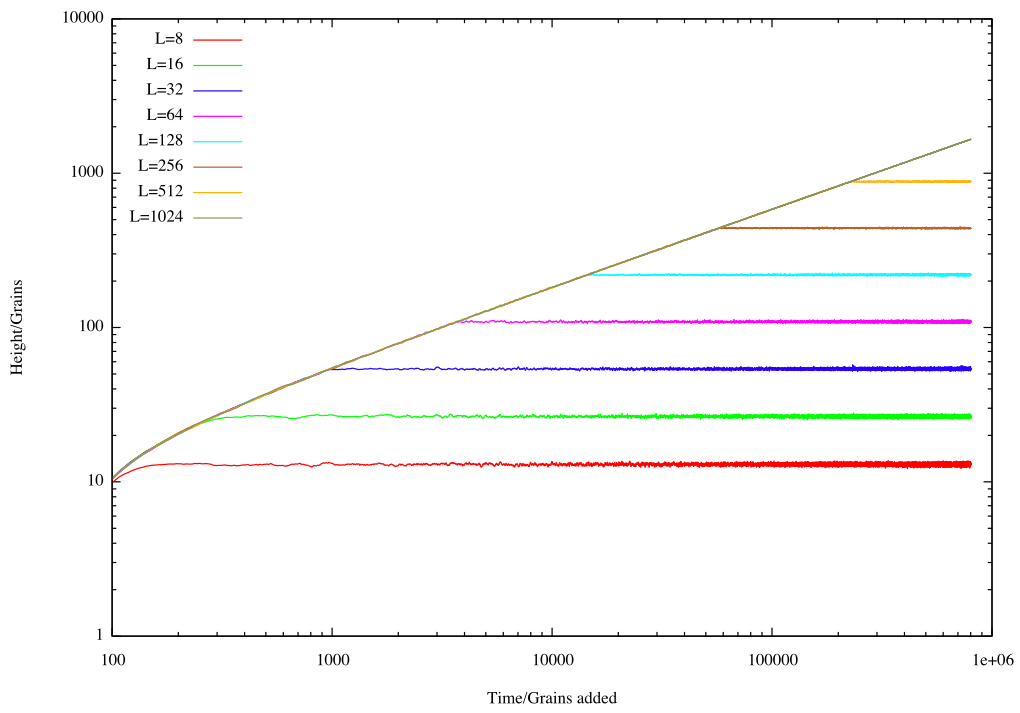
\includegraphics[height=60mm]{hvt-runningmean.png}
  \captionof{figure}{Running mean height of the pile as a function of time, starting from an empty lattice, after the cross over time the system goes from the set of transient configurations to a steady state which are the recurrent configurations.}
\end{center}

\begin{center}
  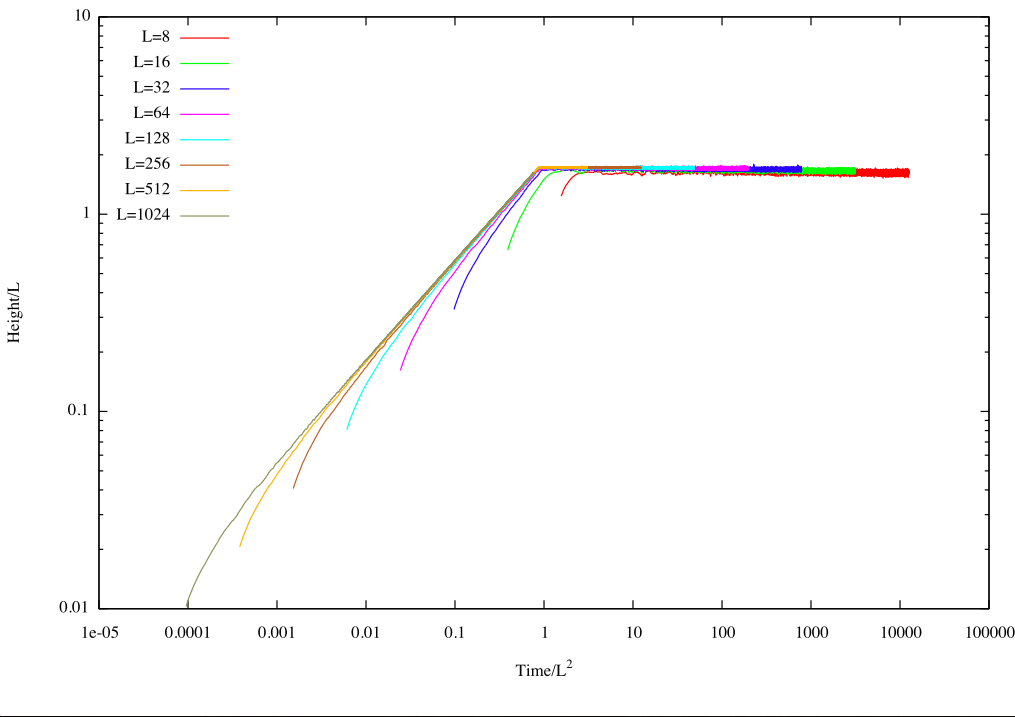
\includegraphics[height=60mm]{datacollapse.png}
  \captionof{figure}{Running mean height divided by system size of the pile as a function of time divided by the square of system size. Causing the data to collapse for all $L$.}
\end{center}

\end{multicols}

The heights in the steady state must scale with $L$ because the minimum height, corresponding to the recurrent configuration $z_i=1 \forall i$ scales with $L$ and the maximum height corresponding to the recurrent configuration $z_i = 2 \forall i$ scales with $2L$\footnote{See appendix I}, so that
\[
L\leq h_{\text{steady state}} \leq 2L
\] 
so that if $ h_{steady state} \propto L^{\tau} $ then if $\tau \neq 1$ the height will eventually hit the maximum or minimum theoretical value and from that point scale with $L^1$. If the time scaling and height scaling behaves as predicted in theory then the data will collapse if the running mean is transformed:
\[
\widetilde{h}(t) = \bar{h} (t L^{-2} ) L^{-1}
\]
where $\bar{h}$ is the running mean, and $\widetilde{h}$ is the transformed running mean in order to make the data collapse.

Since the data collapses it can be concluded that the cross over times scale with $L^2$ and the steady state height with $L$

\subsection{Height distribution and Local Slopes During Steady State}
Since the heights scale with $L$, it is also reasonable to assume that $\langle h \rangle$ also scale with $L$. For the probability mass function of threshold slopes chosen for a random site, then it would be expected that for $z_{th}^i \in \{ 1,2 \} $
\[
\langle h \rangle = L \sum_i p(z_i) z_i = L \times (2-p_{z_{th} = 1} ) 
\]
where $p_{z_{th} = 1} $ is the assignment of the threshold defined in the Oslo algorithm. However this is not the case once the system has reached the attractor of the dynamics. The reason is that sites where $z_{th}^i = 1$ get reassigned a new value more frequently, so that the probability mass function of threshold slopes chosen at random is skewed towards higher thresholds. This isn't the case for a system size $L=1$, where the reassignment goes back to the distribution that is naively expected. If the values are randomly assigned in the Oslo algorithm,
\[
z_i^{th} \to \left\{ \begin{matrix} 1 & \quad \text{with probability } p \\ 2 & \quad \text{with probability } 1-p \end{matrix} \right.
\]
For $p=0.5$, the value of the mean slope measured out to be $\langle z \rangle=1.7287 \pm 0.0007$, measured from the simulation.
\begin{multicols}{2}
\begin{center}
  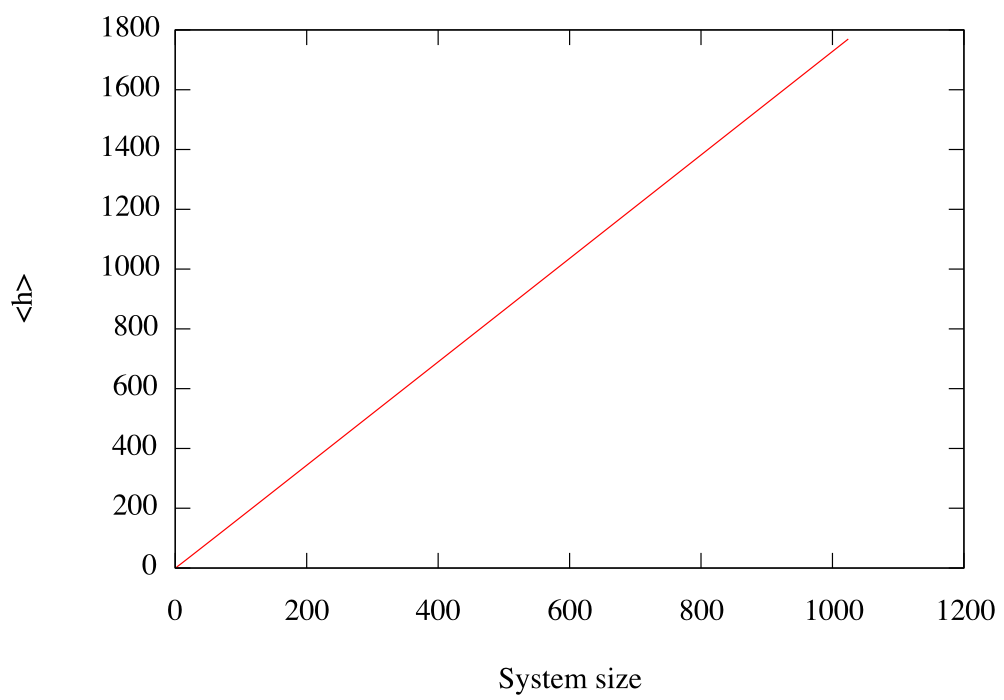
\includegraphics[height=60mm]{mvl.png}
  \captionof{figure}{Mean height as a function of system size.}
\end{center}
\begin{center}
  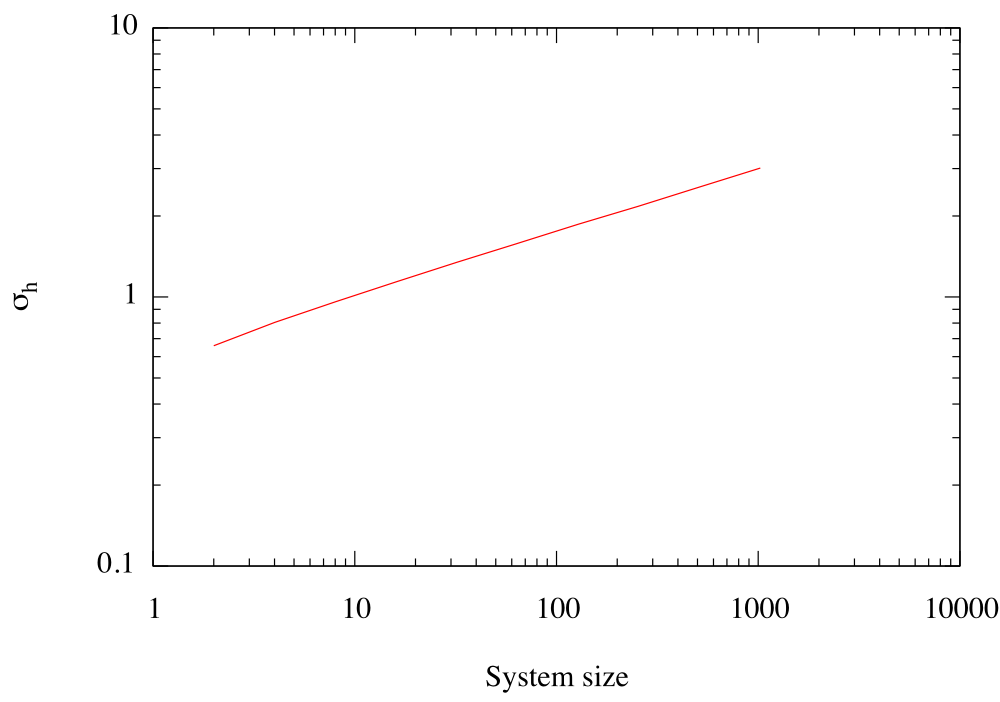
\includegraphics[height=60mm]{svl.png}
  \captionof{figure}{Standard deviation of height as a function of system size.}
\end{center}
\end{multicols}
The standard deviation of the height was found to scale as $\sigma_h \sim L^{0.241 \pm 0.002}$. The Scaling of the standard deviation of the slope can be deduced by:
\[
\sigma_z \sim \sqrt{\langle h^2 L^{-2} \rangle - \langle h \rangle^2  L^{-2}} = L^{-1} \sigma_h
\]
So that $\sigma_z \sim  L^{-0.759 \pm 0.002}$. The average slope stays the same across all length scales, the standard deviation of the local slopes tend to zero as $L \to \infty$.

The probability distributions of the heights can be collapsed for different system sizes to show these results.
\[
\widetilde{P}(h)=L^{0.245} P(( h-\langle z \rangle L) L^{-0.245})
\]
Where $\widetilde{P}(h)$ is the transformed probability in order to collapse the data for different system sizes.
\begin{multicols}{2}
\begin{center}
  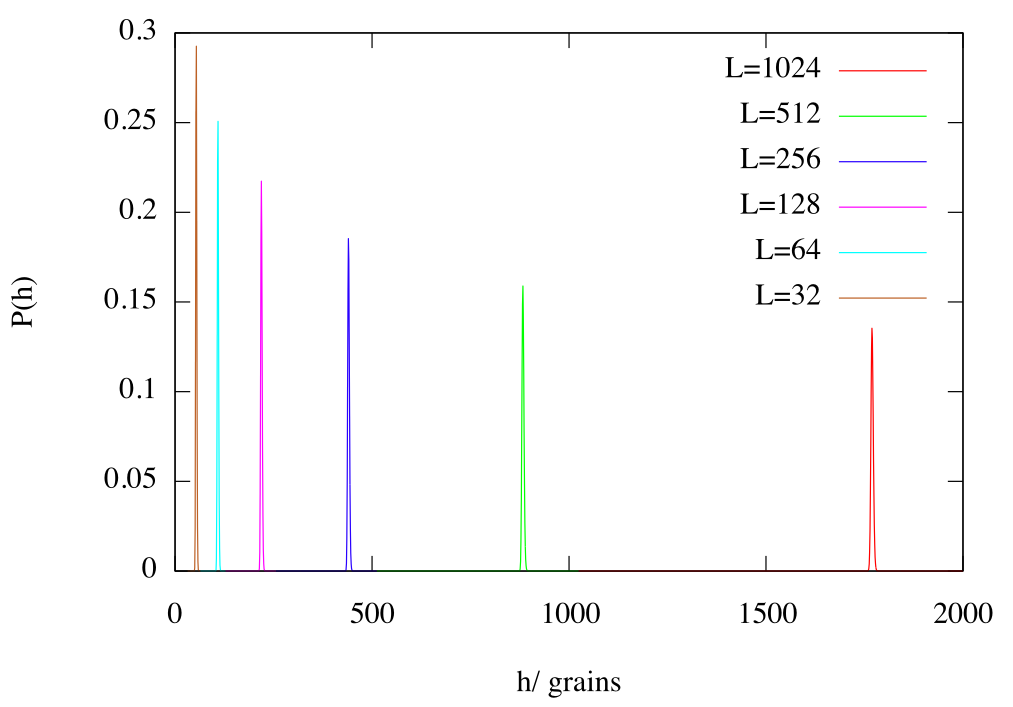
\includegraphics[height=60mm]{pvh.png}
  \captionof{figure}{Probability of height for different system sizes}
\end{center}
\begin{center}
  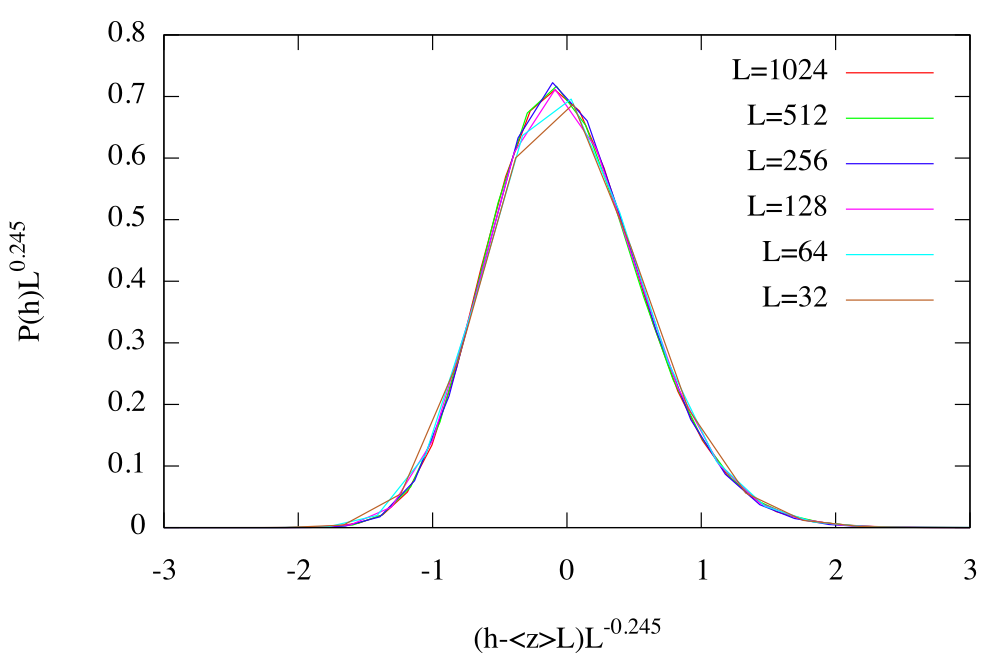
\includegraphics[height=60mm]{pvhb.png}
  \captionof{figure}{$L^{0.245} P$ as a function of $( h-\langle z \rangle L) L^{-0.245}$}
\end{center}
\end{multicols}
Since the transformation caused the data to collapse for different system sizes, it implies that the values found for the scaling of the standard deviation and mean with system size are correct.

\subsection{Avalanche Size}
\begin{center}
  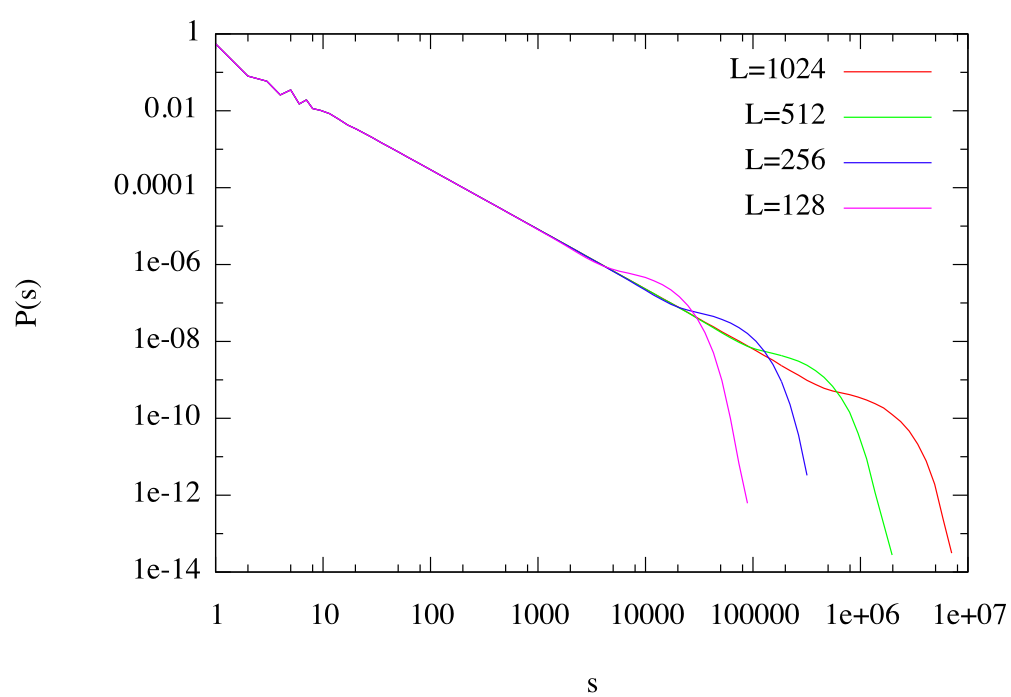
\includegraphics[height=100mm]{pvsbl.png}
  \captionof{figure}{Probability of avalanche size for different system sizes. The linear portions define the scaling region in which $1 \ll s \ll s_c(L) $, which is well approximated by a power law decay $P(s; L) \propto s^{-\tau_s} $. In this region there is no typical avalanche size, up to the cut off $s_c$ which increases with system size, as it is caused by the fact that the system is not infinite, in an infinite system the scaling region would also span to infinity, and the avalanche sizes would be scale free. The humps at the tail end of each probability density function are caused by the frequency being pushed up by avalanches that would have been larger if the system size was not limited. }
\end{center}

The finite scaling ansatz for the avalanche-size probability is given by 
\begin{align*}
P(s,L) &= a s^{-\tau_s} \mathcal{G} (s/s_c) \\ 
s_c (L ) &= b L^D
\end{align*}
Using moment analysis the $k$th moment scales as
\[
\langle s^k \rangle \propto L^{D(1+k-\tau_s)}
\]
The maximum size of an avalanche in the set of recurrent configurations scales as\footnote{see appendix I}
\[
s_{\text{max}} = \frac{L^3}{6} (1 + \mathcal{O} ( L^{-1}) )
\]
However, the minimum avalanche size is $0$ so be the same arguments as in the previous section imply the mean ($k=1$ moment) avalanche sizes scales such that
\[
0 < D(2-\tau_s )\leq 3
\]
and the cut off sizes scale such that
\[
0 < D \leq 3
\]
Using regression on the scaling region of the log-log plot of the probability density function, the exponent $\tau_s$ is
\[
\tau=1.57 \pm 0.02
\]
Plotting $s^{\tau_s} P(s)$ vs $s$ will therefore cause the scaling region to collapse.
Using the cut-off regions, the scaling with system size of the cut off regions $D$ was estimated at
\[
D=2.13 \pm 0.13
\]
checking this using data collapse again should cause the cut off regions to align.
\begin{multicols}{2}
\begin{center}
  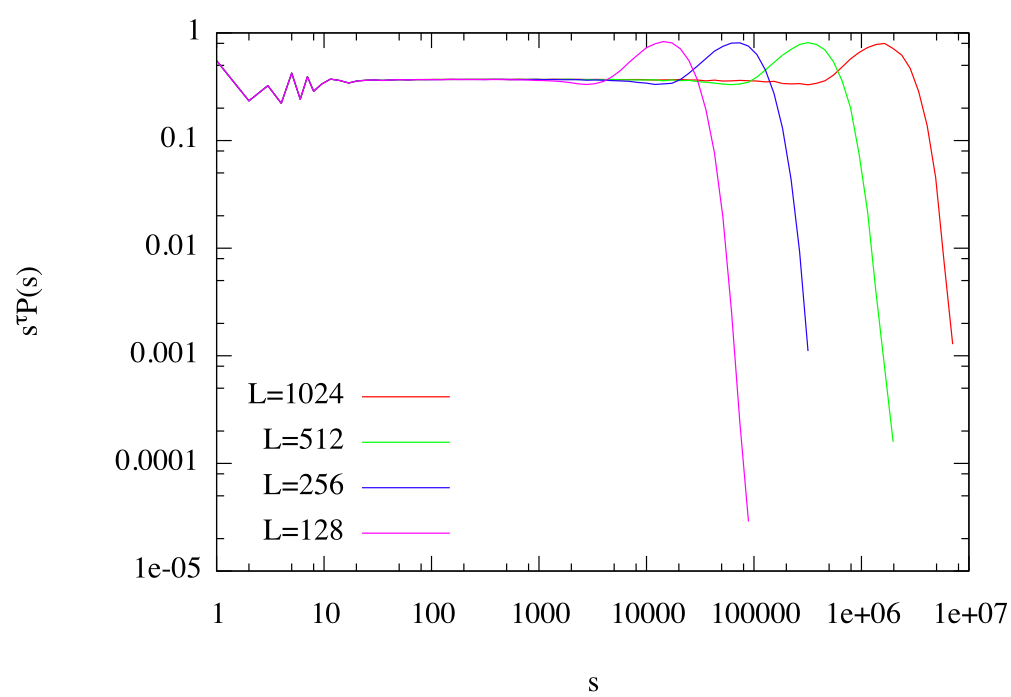
\includegraphics[height=60mm]{pvsblc1.png}
  \captionof{figure}{ $s^{\tau_s} P(s)$ as a function of $s$. $\tau_s = 1.55$ was used to obtain the best collapse, $\tau_s$ is within estimated errors }
\end{center}
\begin{center}
  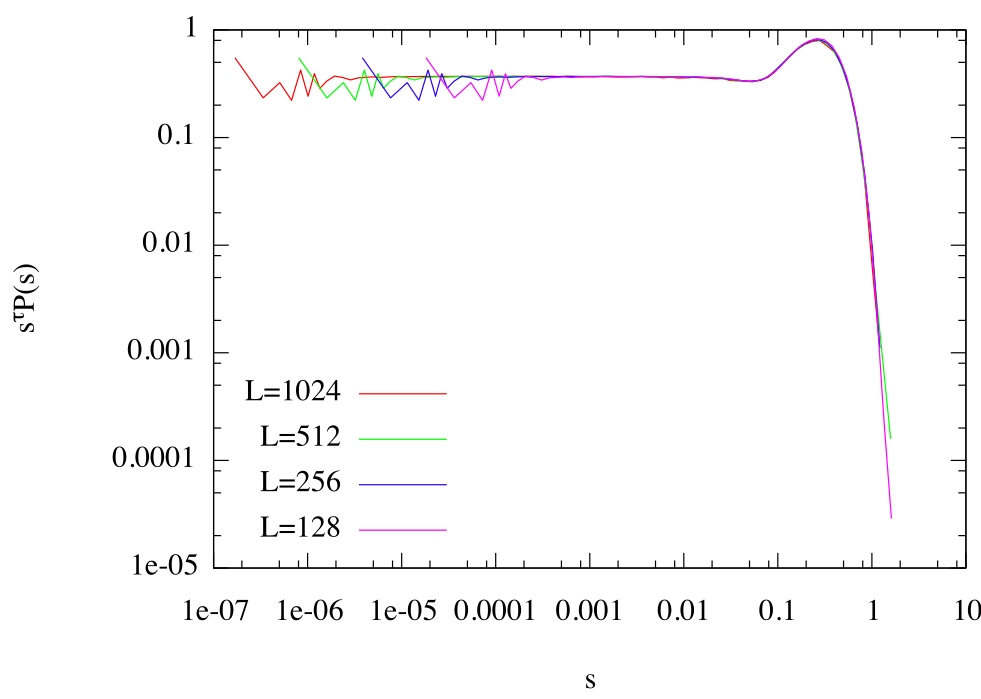
\includegraphics[height=60mm]{pvsblc2.png}
  \captionof{figure}{ $s^{\tau_s} P(s)$ as a function of $sL^{-D}$. $\tau_s = 1.55$, $D=2.25$ was used to obtain the best data collapse, $\tau_s$ and $D$ are within estimated errors }
\end{center}
\end{multicols}
The $k$th moment should scale as 
\[
\langle s^k \rangle \propto L^{2.25(k-0.55)}
\]
Measuring $\langle s^k \rangle$ directly and plotting on log scale to find that the scaling for a given $k$, the predicted values are within the error of the measured values.
\begin{center}
    \begin{tabular}{|l|l|l|}
    \hline
    Moment & Exponent with which the moment scales as & $2.25(k-0.55)$ \\ \hline
    $\langle s \rangle$ & $0.9995 \pm 0.0002$ & $1.0125$\\ \hline
    $\langle s^2 \rangle$ & $3.19 \pm 0.01$ & $3.2625$\\ \hline
    $\langle s^3 \rangle$ &  $5.40 \pm 0.01$ & $5.5125$\\ \hline
    $\langle s^4 \rangle$ &  $7.62 \pm 0.02$ & $7.7625$\\ \hline
    $\langle s^5 \rangle$ &  $9.83 \pm 0.02$ & $10.0125$\\ \hline
    $\langle s^6 \rangle$ &  $12.04 \pm 0.04$ & $12.2625$\\ \hline
    \end{tabular}
\end{center}
The moment analysis suggests that the estimated values for $D$ and $\tau_s$ are wrong, it is more likely that the values obtained from moment analysis are correct since the error values are lower.

\begin{multicols}{2}
\begin{center}
  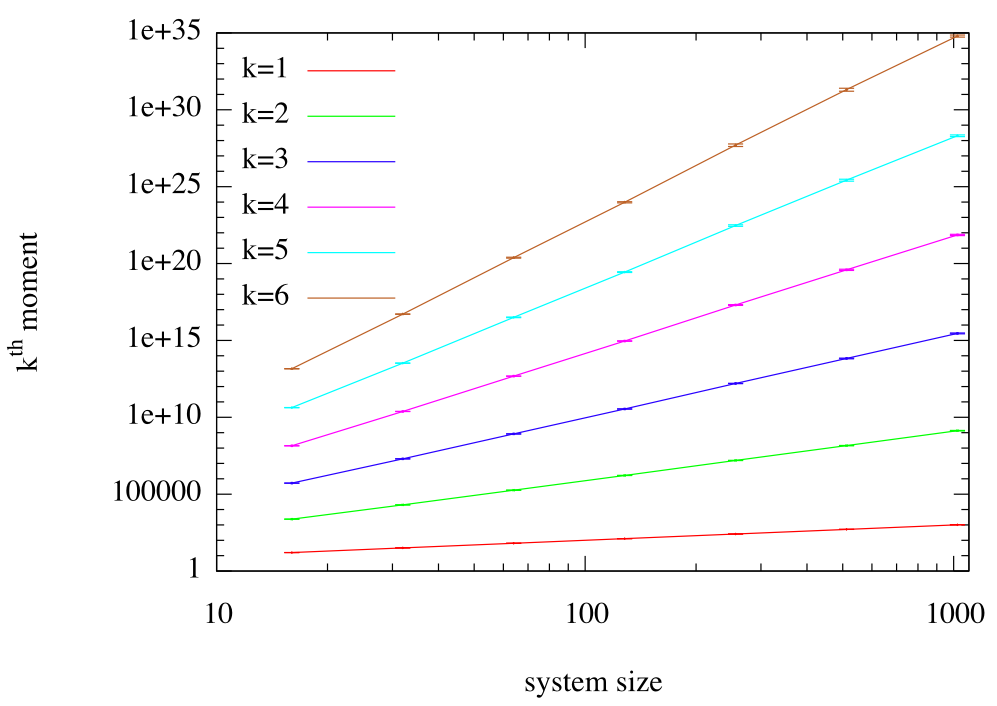
\includegraphics[height=60mm]{movl.png}
  \captionof{figure}{  $\langle s^k \rangle $ as a function of system size }
\end{center}
\begin{center}
  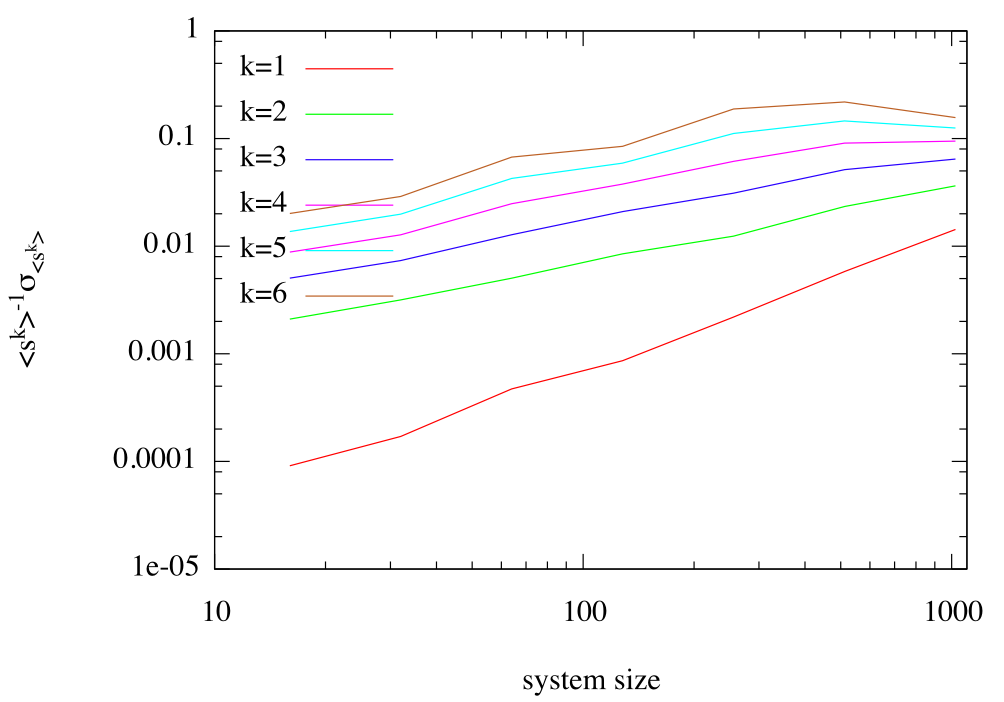
\includegraphics[height=60mm]{smovl.png}
  \captionof{figure}{ Percentage Error of $\langle s^k \rangle $ as a function of system size}
\end{center}
\end{multicols}
The estimates for the critical exponents using moment analysis is found via 
\[
\begin{pmatrix}
\sigma_{\text{est}} \\
\tau_{\text{est}} \sigma_{\text{est}}
\end{pmatrix} =
\left[
\begin{pmatrix}
2 & 3 & \cdots & 6 \\
-1 & -1 & \cdots & -1
\end{pmatrix}
\begin{pmatrix}
2 & -1 \\
3  & -1 \\
\vdots & \vdots \\
6 & -1
\end{pmatrix}
\right]^{-1}
\begin{pmatrix}
2 & 3 & \cdots & 6 \\
-1 & -1 & \cdots & -1
\end{pmatrix}
\begin{pmatrix}
0.9995 \\
3.19 \\
\vdots \\
12.04
\end{pmatrix}
\]
\[
\begin{pmatrix}
\sigma_{\text{est}} \\
\tau_{\text{est}} \sigma_{\text{est}}
\end{pmatrix} =\begin{pmatrix}
2.20979 \\
3.43079
\end{pmatrix} 
\]
so, $\sigma_{\text{est}} = 2.20979$ and $\tau_{\text{est}} = 1.542$. 
\begin{center}
  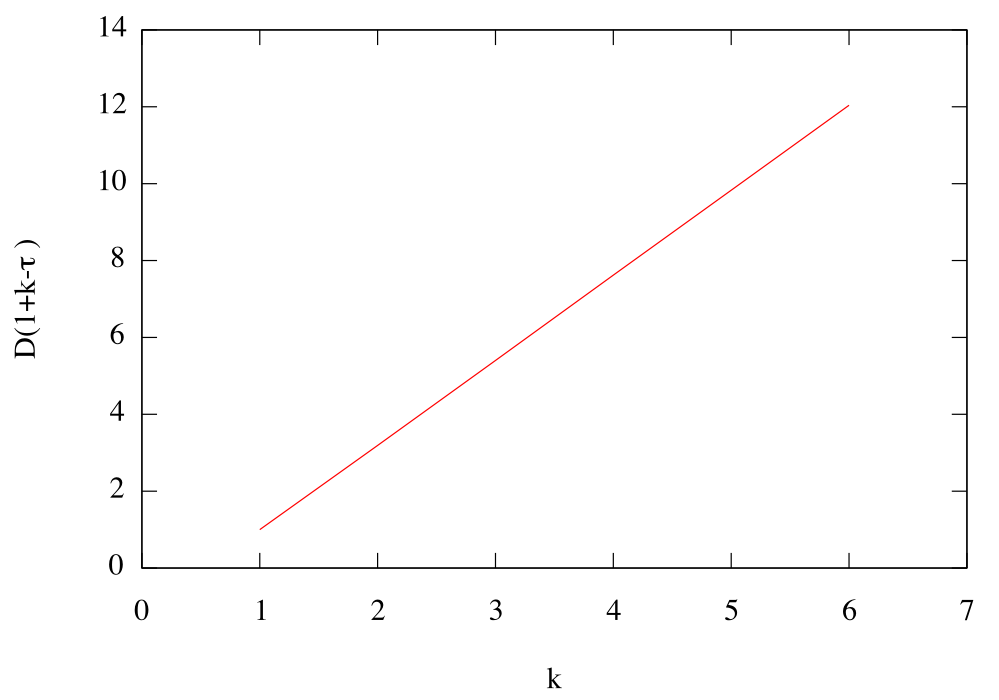
\includegraphics[height=60mm]{movl2.png}
  \captionof{figure}{ $D(1+k - \tau )$ as a function of $k$. Using a machine-learning regression algorithm by fitting $f(x)=m(x+1-b)$, (so that $b_{\text{final}}=\tau_{\text{est}}$ and $m_{\text{final}} = D_{est}$ ) results with $D_{\text{est}} = 2.20979 \pm 0.001968$ and $\tau_{\text{est}}=1.553 \pm 0.003 $. Moment analysis has produced consistent results with greater accuracy.}
\end{center}
\subsection{Drop Sizes}
\begin{center}
  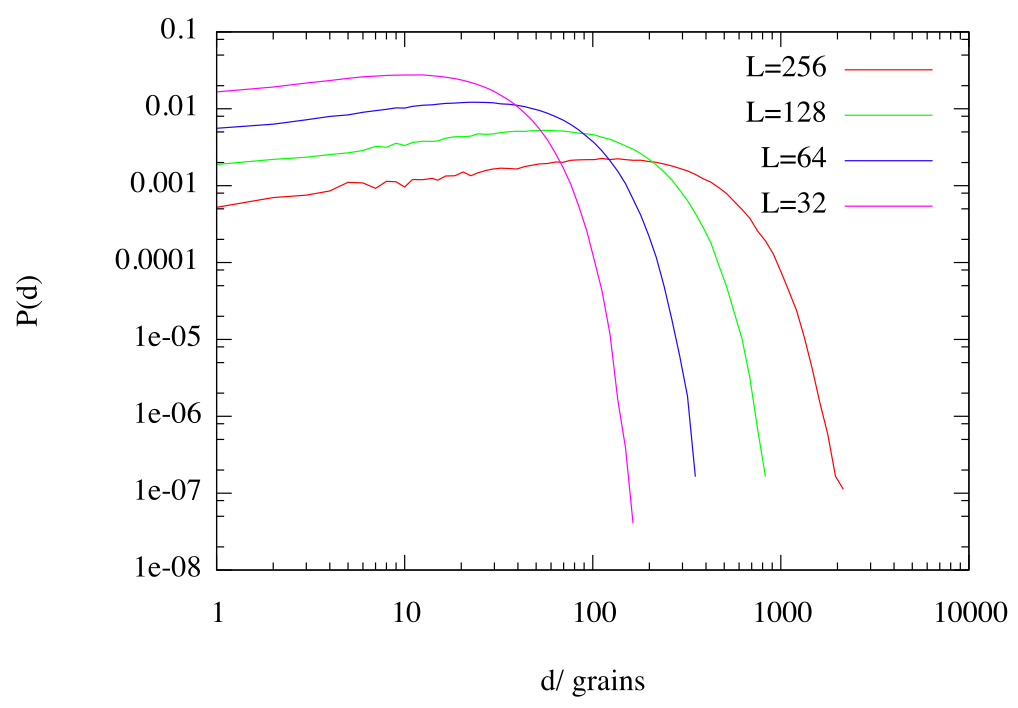
\includegraphics[height=60mm]{pvd.png}
  
  \captionof{figure}{Probability density as a function of drop size. The drop size behaves sale free up to an exponential cut off, unlike the fat tailed probability distributions of the avalanche sizes. }
\end{center}
The drop sizes appear to have an exponential cut off. We can use the same scaling ansatz as before. Using moment analysis:
\begin{center}
    \begin{tabular}{|l|l|}
    \hline
    Moment & Exponent with which the moment scales as  \\ \hline
    $\langle d \rangle$ & $1.14 \pm 0.03$\\ \hline
    $\langle d^2 \rangle$ & $2.31 \pm 0.05$ \\ \hline
    $\langle d^3 \rangle$ &  $3.50 \pm 0.06$ \\ \hline
    $\langle d^4 \rangle$ &  $4.71 \pm 0.08$ \\ \hline
    $\langle d^5 \rangle$ &  $5.93 \pm 0.09$ \\ \hline
    $\langle d^6 \rangle$ &  $7.2 \pm 0.1$ \\ \hline
    \end{tabular}
\end{center}

\begin{multicols}{2}
\begin{center}
  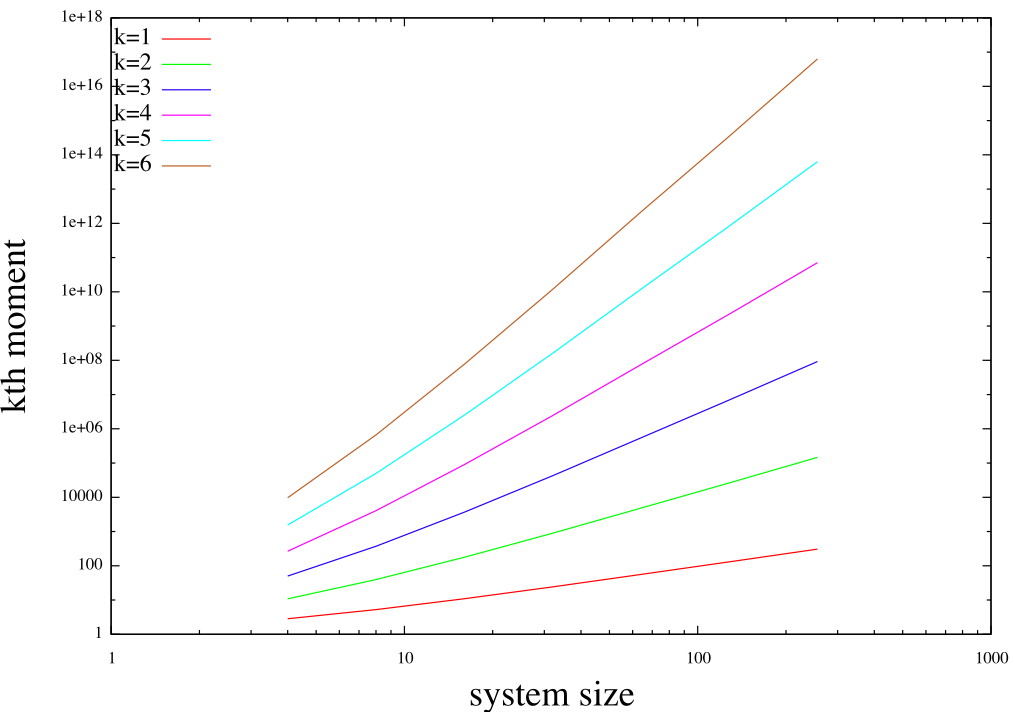
\includegraphics[height=60mm]{dmovl.png}
  \captionof{figure}{kth moment of the drop size versus system size}
\end{center}
\begin{center}
  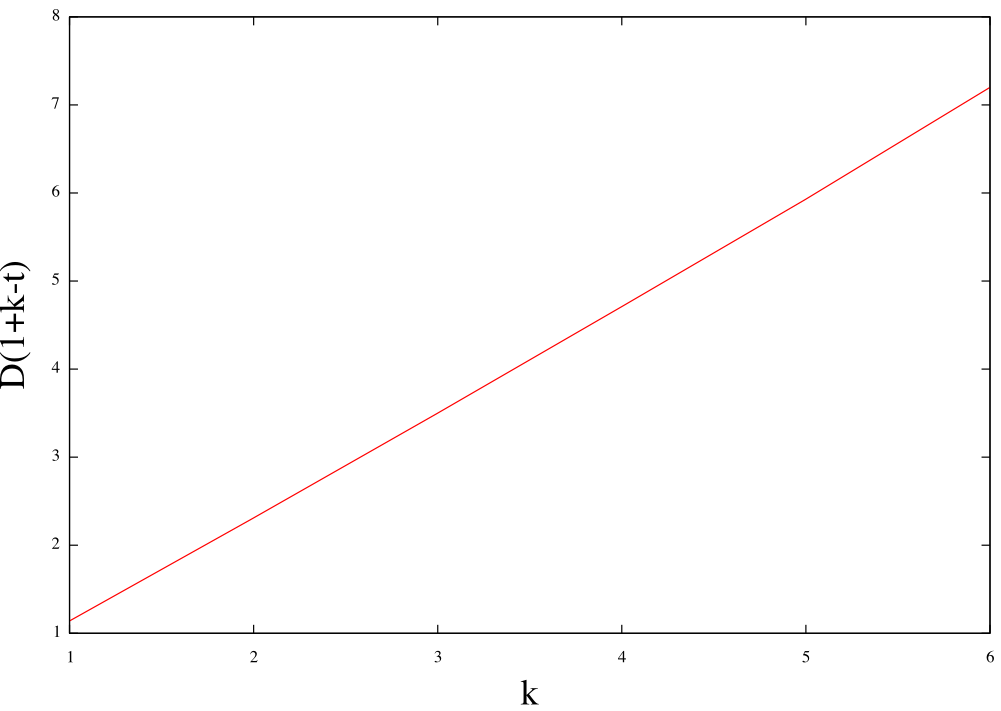
\includegraphics[height=60mm]{dmovl2.png}
  \captionof{figure}{$D(1+k - \tau )$ as a function of $k$. Using a machine-learning regression algorithm by fitting $f(x)=m(x-1-b)$, (so that $b_{\text{final}}=\tau_{\text{est}}$ and $m_{\text{final}} = D_{est}$ ) results with $D_{\text{est}} = 1.21057 \pm 0.008218$ and $\tau_{\text{est}}=1.09 \pm 0.03 $. Moment analysis has produced consistent results with greater accuracy.}
\end{center}
\end{multicols}
\begin{center}
  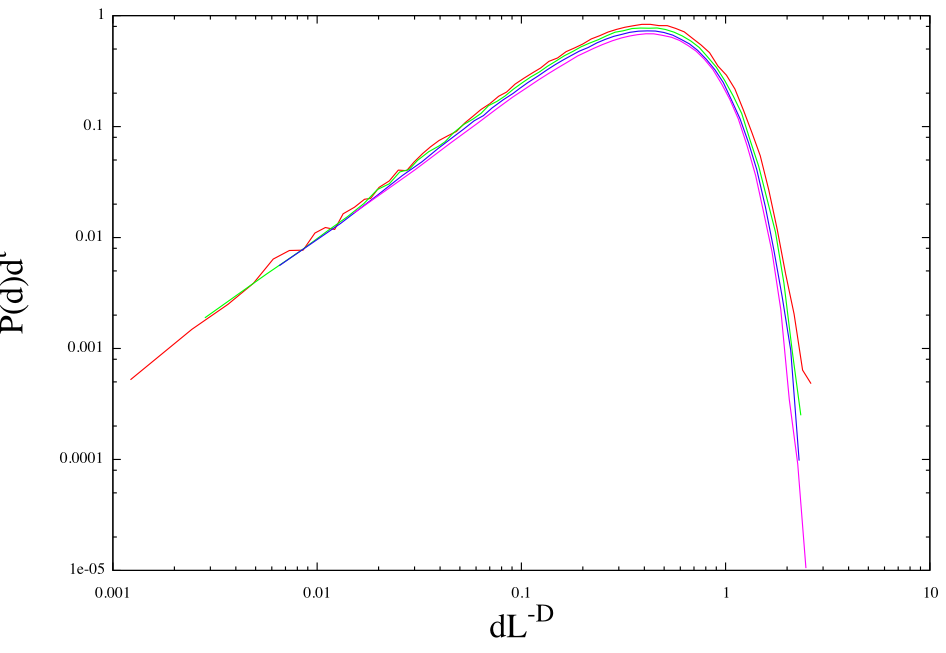
\includegraphics[height=60mm]{datac.png}
  \captionof{figure}{data collapsed drop sizes}
\end{center}

%------------------------------------------------DISCUSSION

\section{Discussion}

The $L=1$ case behaves differently to other system sizes since there is no interaction with other sites, so that the threshold slope is randomly assigned. For $L>1$ the distribution of threshold slope is skewed towards higher thresholds due to the higher thresholds being reassigned less frequently. A greater number of high threshold sites do not make sense, since these are more unstable, theoretically they should be more improbable. The model could be adjusted, instead of choosing the threshold slopes with uniform probability, it would perhaps be more realistic to choose threshold slopes weighted towards lower thresholds.



%------------------------------------------------CONCLUSION

\section{Conclusion}
In conclusion we have observed that the Oslo model self-organises such that there is no typical scale for avalanche sizes. with cut-offs occurring due to finite system size, there also appears to be  regions near the tail end where there would otherwise be larger avalanches if the system size is taken to infinity. The height of the system obviously increases to infinity, but the local slope tends to an average of $1.7287\pm 0.0007$. Drop sizes also have a region which is scale free which increases with system size, but ends in an exponential cut off.


%----------------------------------------------------------------------------------------
%	APPENDICES
%----------------------------------------------------------------------------------------
\clearpage 

\section{Appendices}
\subsection{Theoretical limits on $h(t,L)$ and $s(t,L)$}
The maximum value for the height would be if every single site $i$ has the maximum possible threshold. $z_i (t) = 2 \; \forall i$. Hence:
\[
h_{\text{max}} = \sum_{i=1}^L 2 = 2L
\]
and the theoretical minimum value for the height during the steady state is when $z_i (t) = 1 \; \forall i$:
\[
h_{\text{min}} = L
\]
The theoretical minimum avalanche size would trivially be 0. The theoretical maximum avalanche size would be if the pile starts in the configuration $z_i (t) = 2 \; \forall i$ after a single grain is added the pile goes into the configuration where $z_i (t+1) = 1 \; \forall i$. This would entail $L-(i-1)$ topplings from each grain at site $i$. Each grain at site i also has $L-(i-1)$ grains. Hence:
\begin{align*}
s_{\text{max}}& = L+ \sum_{i=1}^L (L-(i-1))^2 \\
&=L+ \sum_{i=0}^L (L-i)^2\\
&= L+ \sum_{i=0}^L i^2 \\
&= L+ \frac{L}{6} (2L+1) (L+1) \\
&= \frac{L^3}{6} ( 1 + \mathcal{O}(L^{-1} ) )
\end{align*}
Where the additional $L$ comes from the toppings of the grain added to the system $z_i = 2 \forall i$. 

	The maximum theoretical drop size also corresponds to $z_i (t) = 2 \; \forall i$ going to a configuration of $z_i (t+1) = 1 \; \forall i$ after a single grain is added. Each site $i$ has lost $L-(i-1)$ grains, as well as the grain added so that
\[
d_{max} = \frac{L}{2} (L+1) + 1\sim \frac{L^2}{2} ( 1 + \mathcal{O}(L^{-1} ) )
\]

\subsection{Solving for the Critical Exponents from Moment Analysis}
For a finite scaling ansatz $P(x,y) = a x^{-\tau} \mathcal{G} (x/ y^{\sigma} )$.
Measuring the $k$th moment $\langle x^k \rangle$ and it's scaling with $y$ will result in $n$ equations for the exponents $\tau$ and $\sigma$:

\[
\underline{\underline{A}}
\underline{x} =
\begin{pmatrix}
2 & -1 \\
3  & -1 \\
\vdots & \vdots \\
n & -1
\end{pmatrix}
\begin{pmatrix}
\sigma \\
\tau \sigma
\end{pmatrix}
= \begin{pmatrix}
a_1 \\
a_2 \\
\vdots \\
a_n
\end{pmatrix}
\]
Where $a_i$ is the measured exponent with which the $i$th moment scales. Most likely, the vector $\underline{a} \not\in \text{Col}(\underline{\underline{A}} )$. In which case we find the projection of $\underline{a}$, $\underline{\underline{P}}_A \underline{a}$ onto the column space of  $\underline{\underline{A}}$, instead solving the equation $\underline{\underline{A}}\underline{x_{\text{est} }} = \underline{\underline{P}}_A \underline{a}$. The difference $ \underline{a}-\underline{\underline{A}}\underline{x_{\text{est} }}$ must be orthogonal to $\text{Col}(\underline{\underline{A}})$ so that $\underline{a}-\underline{\underline{A}}\underline{x} \in \text{Null} (\underline{\underline{A}}^T)$:
\[
\underline{\underline{A}}^T( \underline{a}-\underline{\underline{A}}\underline{x}) =0
\]
Solving for this gives:
\[
\begin{pmatrix}
\sigma_{\text{est}} \\
\tau_{\text{est}} \sigma_{\text{est}}
\end{pmatrix}=
(\underline{\underline{A}}^T\underline{\underline{A}})^{-1} \underline{\underline{A}}^T \underline{a}
 = \underline{\underline{A}}_{\text{left}}^{-1} \underline{a} 
\]
$\underline{\underline{A}}^T\underline{\underline{A}}$ is always invertible if the columns of $\underline{\underline{A}}$ are linearly independent. The best solution ends up being obtained by using the left inverse of the matrix. Plotting $a_{k}$ vs $k$ and doing regression, is mathematically equivalent to using the left inverse. The residuals can be calculated by $||\underline{a}- \underline{\underline{P}}_A\underline{a} ||$ (using the euclidean norm this is equivalent of the rms of the residuals).

\subsection{Data Binning Graphs}
\begin{multicols}{2}
\begin{center}
  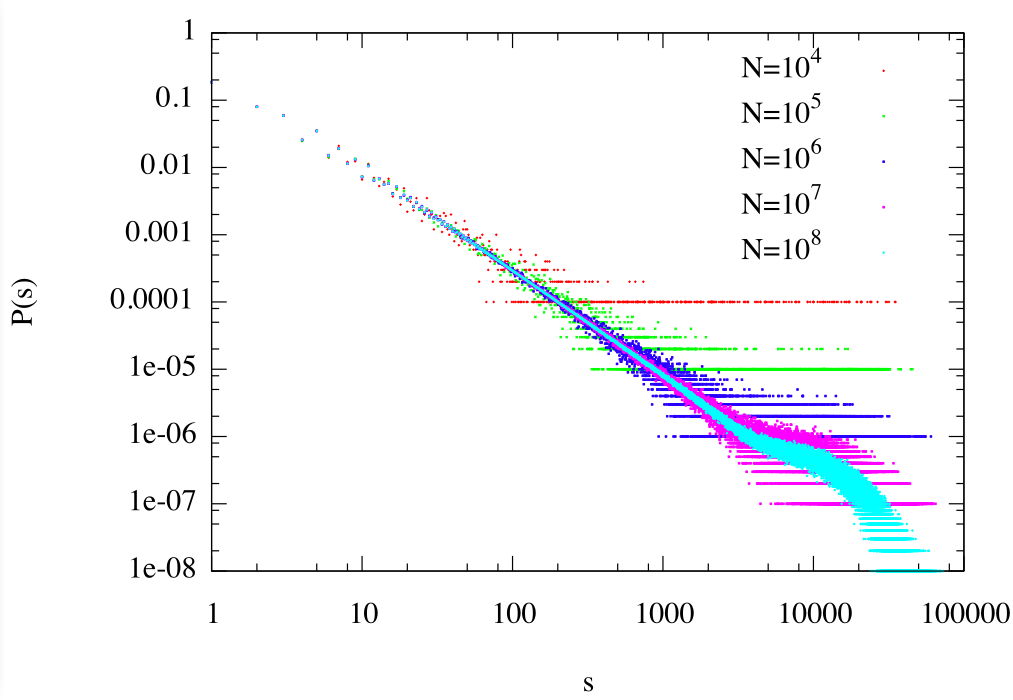
\includegraphics[height=55mm]{lb1.png}
  \captionof{figure}{Probability mass function estimates of avalanches for different numbers of total avalanches $N$ in the Oslo model, for a system size $L=128$.}
\end{center}
\begin{center}
  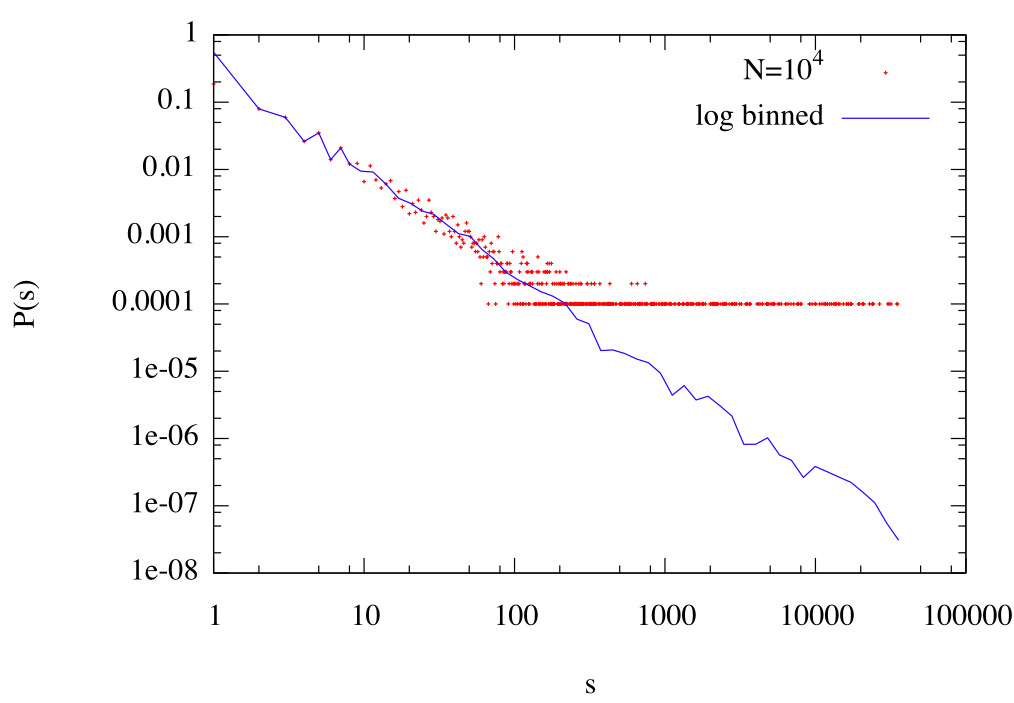
\includegraphics[height=55mm]{lb2.png}
  \captionof{figure}{Probability mass function estimates of avalanches for different numbers of total avalanches $N$ in the Oslo model using log binning for $10^4$ total avalanches.}
\end{center}
\end{multicols}
\begin{multicols}{2}
\begin{center}
  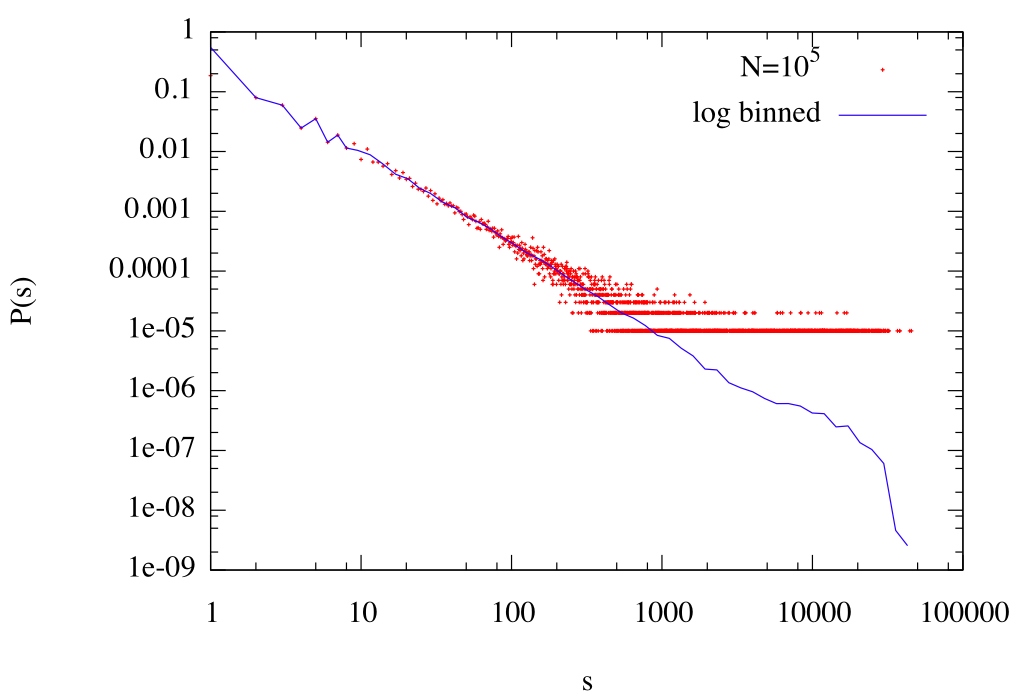
\includegraphics[height=55mm]{lb3.png}
  \captionof{figure}{Probability mass function estimates of avalanches for different numbers of total avalanches $N$ in the Oslo model using log binning for $10^5$ total avalanches.}
\end{center}
\begin{center}
  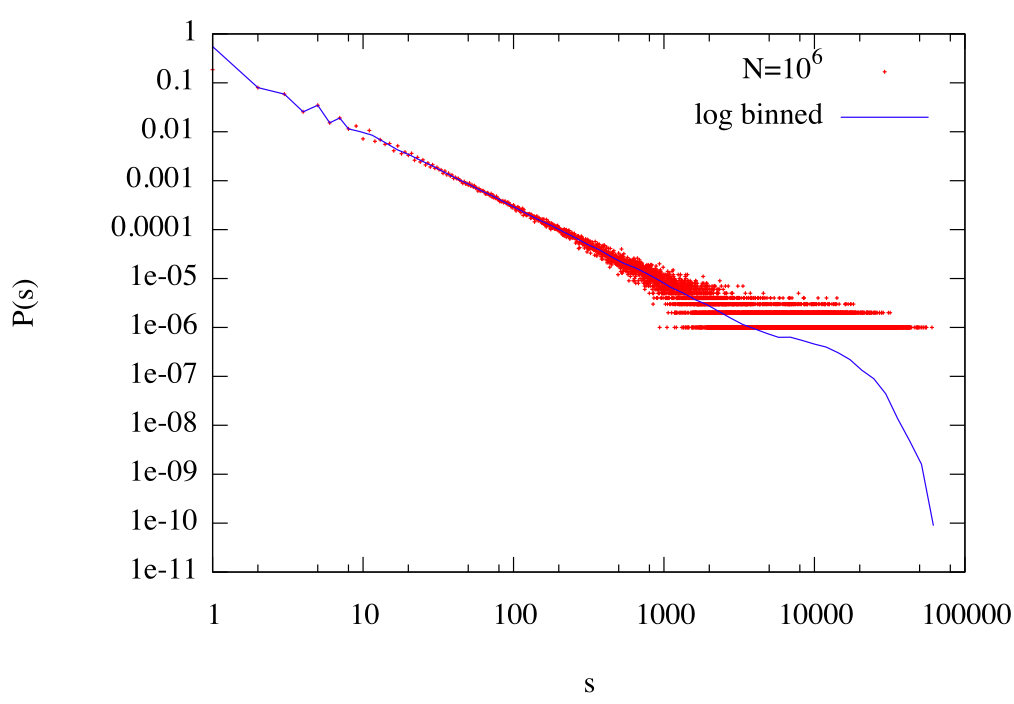
\includegraphics[height=55mm]{lb4.png}
  \captionof{figure}{Probability mass function estimates of avalanches for different numbers of total avalanches $N$ in the Oslo model using log binning for $10^6$ total avalanches.}
\end{center}
\end{multicols}
\begin{multicols}{2}
\begin{center}
  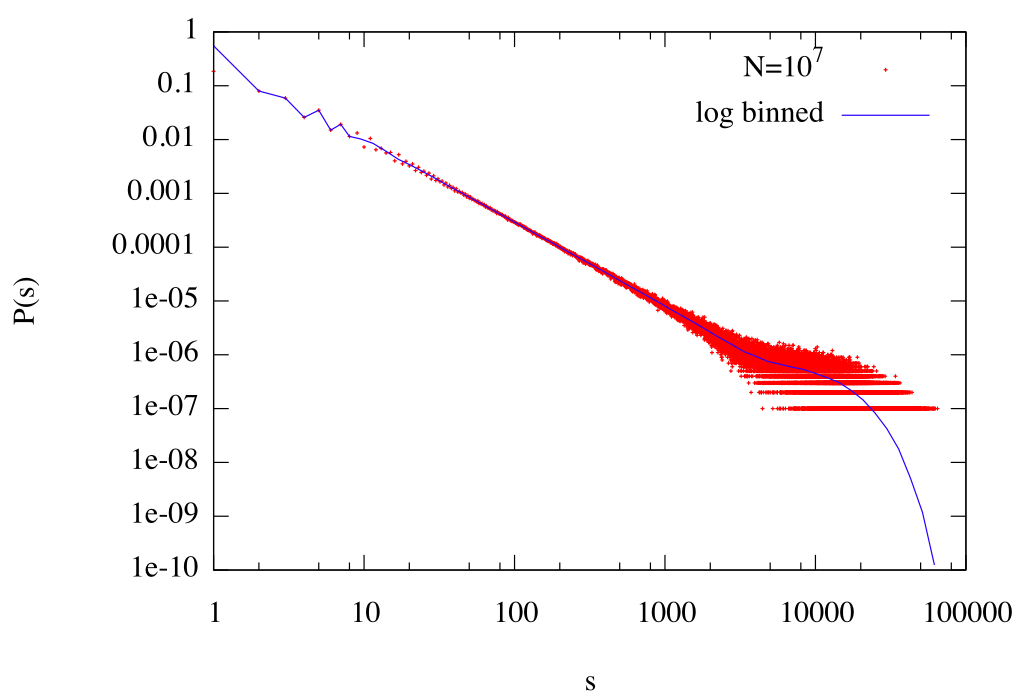
\includegraphics[height=55mm]{lb5.png}
  \captionof{figure}{Probability mass function estimates of avalanches for different numbers of total avalanches $N$ in the Oslo model using log binning for $10^7$ total avalanches.}
\end{center}
\begin{center}
  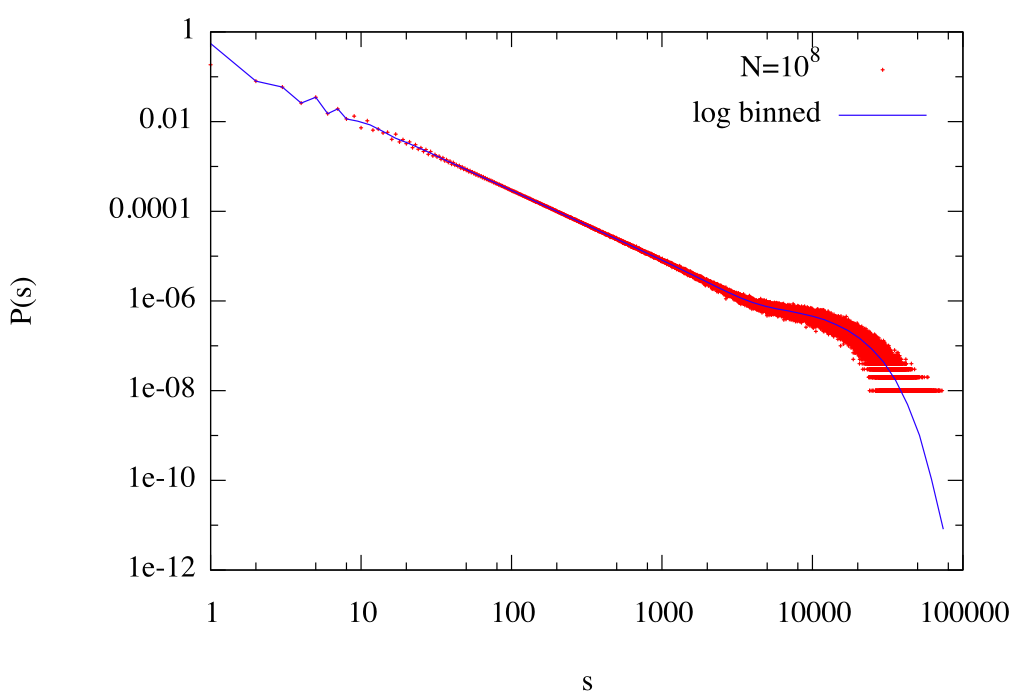
\includegraphics[height=55mm]{lb6.png}
  \captionof{figure}{Probability mass function estimates of avalanches for different numbers of total avalanches $N$ in the Oslo model using log binning for $10^8$ total avalanches.}
\end{center}
\end{multicols}


%----------------------------------------------------------------------------------------
%	REFERENCE LIST
%----------------------------------------------------------------------------------------
\clearpage
\begin{thebibliography}{99} % Bibliography - this is intentionally simple in this template

\bibitem[1]{cc}
\newblock Christensen, Kim, and Nicholas R. Moloney. 
\emph{Complexity \& Criticality.}

\newblock  Imperial College Press, 2005


 
\end{thebibliography}

%----------------------------------------------------------------------------------------



\end{document}
